\documentclass[UTF8,a4paper]{ctexart}
\usepackage{geometry} % 设置页边距,页面大小
\geometry{left=2.5cm,right=2.0cm,top=2.50cm,bottom=2.0cm}
\linespread{1.3}%调整行间距
\usepackage{graphicx} % 引入图片
%\usepackage[justification=centering]{caption} % 图片的caption居中
\usepackage[indent]{caption} % 设置图片的 caption 换行缩进
% Inkscape矢量图
\usepackage{import}
\usepackage{xifthen}
\usepackage{pdfpages}
\usepackage{transparent}
\usepackage{calc} %调整大小


\pagestyle{plain}    % 没有页眉,页脚是居中的页码;
\usepackage{setspace} %行间距
\usepackage{array} %
\usepackage{booktabs} %调整表格线与上下内容的间隔
\usepackage{multirow}
\usepackage{hyperref} %加入书签跳转
\usepackage{fontspec} %引入字体Times New Roman字体
%\setmainfont{Times New Roman}             %设置正文字体为Times New Roman
\usepackage{abstract} % 修改摘要

%\usepackage[fontset=windows]{ctex}
\usepackage{xeCJK} %调用系统中已安装的字体
\setCJKmainfont{SimSun}
\setmainfont{Times New Roman}
%% 支持汉字加粗
\let\heiti\relax % 黑体
\newCJKfontfamily\heiti{SimHei}[AutoFakeBold]
\setCJKsansfont{SimHei}[AutoFakeBold]

\let\songti\relax % 宋体
\newCJKfontfamily\songti{SimSun}[AutoFakeBold]
\setCJKmainfont{SimSun}[AutoFakeBold]  



%% 目录格式设置
\usepackage{tocloft}      %必须这么写,否则会报错
\renewcommand{\contentsname}{\centerline{\Large{\heiti{目\quad\quad 录}}}}
%\renewcommand{\cftchapleader}{\cftdotfill{0.6}} %设置chapter条目的引导点间距
\renewcommand{\cftsecleader}{\cftdotfill{0.6}}
\renewcommand{\cftsubsecleader}{\cftdotfill{0.6}}
\renewcommand{\cftsubsubsecleader}{\cftdotfill{0.6}}
%\renewcommand{\cftchapfont}{\hts}    %设置chapter条目的字体
\renewcommand{\cftsecfont}{\heiti}    %设置section条目的字体
\renewcommand{\cftsecfont}{\Large}    %设置section条目的四号
\renewcommand{\cftsubsecfont}{\songti} %设置subsection条目的字体
\renewcommand{\cftsubsecfont}{\large} %设置subsection条目的字体
\renewcommand{\cftsubsubsecfont}{\songti} %设置subsection条目的字体
\renewcommand{\cftsubsubsecfont}{\large} %设置subsection条目的字体


% 数学公式
\usepackage{amsmath}

% 插入代码块
\usepackage{listings}
\usepackage{xcolor}
\lstset{
 %language=bash,                % the language of the code
 columns=fixed,       
% numbers=left,                                        % 在左侧显示行号
% numberstyle=\tiny\color{gray},                       % 设定行号格式
 frame=none,                                          % 不显示背景边框
 backgroundcolor=\color[RGB]{245,245,244},            % 设定背景颜色
 keywordstyle=\color[RGB]{40,40,255},                 % 设定关键字颜色
 numberstyle=\footnotesize\color{darkgray},           
 commentstyle=\it\color[RGB]{0,96,96},                % 设置代码注释的格式
% stringstyle=\rmfamily\slshape\color[RGB]{128,0,0},   % 设置字符串格式
}


% 参考文献
\usepackage{cite}
%%%%%%%%%%%%%%%%%%%%%%%%%%%%%%%%%%%%%%%%%%%%%%%%%%%%%%%%%%%%%%%%%%%%%%%%%%%%%%%%%
%  以下是论文内容
%%%%%%%%%%%%%%%%%%%%%%%%%%%%%%%%%%%%%%%%%%%%%%%%%%%%%%%%%%%%%%%%%%%%%%%%%%%%%%%%%
%  正文
\begin{document}
%% 封面
% 这是封面
\begin{flushright}
\end{flushright}
\begin{center}
    \vskip 1.5cm
    
\includegraphics[scale=0.6]{figs/ncepu.eps}%学校图标
\end{center}
\begin{center}
    \vskip 1.5cm
    
\includegraphics[scale=0.6]{figs/bthesistitle.eps}%毕业设计图标
\end{center}
\begin{center}
  \vskip 2cm
    \fontsize{15}{1} \textbf{题目} \underline{基于Qemu模拟器移植rCore操作系统的开发与实现}
  \vskip 2.5cm
\end{center}
\begin{center}
  \begin{tabular}{l}

    院\quad\quad 系 \underline{\qquad 控制与计算机工程学院 \quad }\\\\
    专\quad\quad 业 \underline{\qquad 计算机科学与技术 \quad\qquad}\\\\
    % \quad 代表空格,输入题目后自己调长度
    班\quad\quad 级 \underline{\qquad\quad 计算1702班 \quad\qquad\quad }\\\\
    学生姓名 \underline{\qquad\qquad 杨秉学\qquad\qquad\qquad}\\\\
    学\quad\quad 号 \underline{\qquad\quad 120171080212 \qquad\qquad }\\\\
    指导教师 \underline{\qquad\qquad\quad 琚贇\qquad\qquad\qquad }\\\\

  \end{tabular}
\end{center}
\begin{center}
        \vskip 2.5cm
    {2021} 年{\quad 六\quad }月{\qquad \qquad }日

\end{center}
\thispagestyle{empty} %去除本页页码
      
%%摘要
%%%% 中文摘要
% 这是中文摘要
\newpage
\pagenumbering{Roman}
\renewcommand{\abstractname}{\heiti{\Large{摘\quad \quad \quad \quad 要}}}
\begin{abstract}
\addcontentsline{toc}{section}{\heiti{\Large{摘 \quad \quad 要}}}    
{\large{RISC-V是一款近年来最为流行的开源指令集架构,被广泛应用于各个场景。Linux也是一个十分流行的开源操作系统内核。本实验采取Qemu虚拟化技术模拟RISC-V指令环境,解决跨平台的模型部署和运行问题。在上面进行移植Linux操作系统,尝试在上面编译安装程序,并对RISC-V指令集以及操作系统,计算机组成原理,计算机体系结构综合知识进行回顾与总结。}}

%\\ \hspace*{\fill} \\  %换行,用空格填充,再换行,即可实现空出一整行的效果,不需任何环境调整
\noindent %取消首航缩进
    {\large{\textbf{关键字}:RISC-V;Qemu;linux;系统移植;}}
\end{abstract}

%%%% 英文摘要
% 这是英文摘要
\newpage
\renewcommand{\abstractname}{\Large \textbf{ABSTRACT}}
\begin{abstract}
{\large{This section is where the summary information is placed.This section is where the summary information is placed.This section is where the summary information is placed.}}

\noindent
\textbf{KEY WORDS:}RISC-V,Qemu,linux
\end{abstract}

%% 目录
\newpage
\tableofcontents
\thispagestyle{empty}

%% 章节
\newpage
\pagenumbering{arabic}
%%%%定制标题样式
%%%%% section
\CTEXsetup[name={第,章 },format={\centering\heiti\zihao{-2}},aftername={\enspace},beforeskip={24bp},afterskip={18bp}]{section} %name选项中不要使用中文逗号 \zihao(-2)字号小二
%%%%% subsection
\CTEXsetup[format={\raggedright\songti\zihao{-3}},aftername={\enspace},beforeskip={24bp},afterskip={6bp}]{subsection}
%%%%% subsubsection
\CTEXsetup[format={\raggedright\songti\zihao{4}},aftername={\enspace},beforeskip={12bp},afterskip={6bp}]{subsubsection}

% 本章节是介绍项目的背景信息
\section{背景}
在“中兴事件”刚过没多久,某国家就开始发起“华为事件”,对我国半导体产业的打击极大,放眼整个产业链,我们国家连一个像样的指令集架构都没有,我们想研究开发产品竟然还需要别人来授权,这是莫大的耻辱。
所以,我觉得是时候我应该研究一下了。
Risc-v是一个最近流行基于RISC指令集架构,类似与软件领域开源的linux一样,Risc-V也有很多领域可以发挥作用。

\newpage  % 课题研究背景和意义
% 本章节是介绍 RISC-V的
\section{计算机组成与设计——基于RISC-V}
本章节是根据 David A. Patterson 的著作\cite{Computer_Organization_and_Design_riscv}以及浙江大学刘鹏博导的公开课\cite{Computer_Organization_and_Design_ZJU}来改编实现的。

\subsection{指令表示方法与指令格式}
如果把计算机比作一个在说话的人,那么指令就是每一个单词,指令集就是全部词汇所构成的词汇表

\subsubsection{R指令}
\textbf{R指令}是用于寄存器与寄存器之间算数运算的

一条R型指令的格式划分如图\ref{fig:R-Format_Instruction_Layout}所示,R型指令可以划分为6个域,其中31-25这7bit宽的是功能码7,24-20这5为是源寄存器2,19-15这5为是源寄存器1,14-12这3bit宽的是功能码3,11-7这5bit宽的目的寄存器rd,6-0这7位宽的操作码(部分规定了该指令是什么指令)。

\begin{figure}[htbp]
  \centering %居中显示
  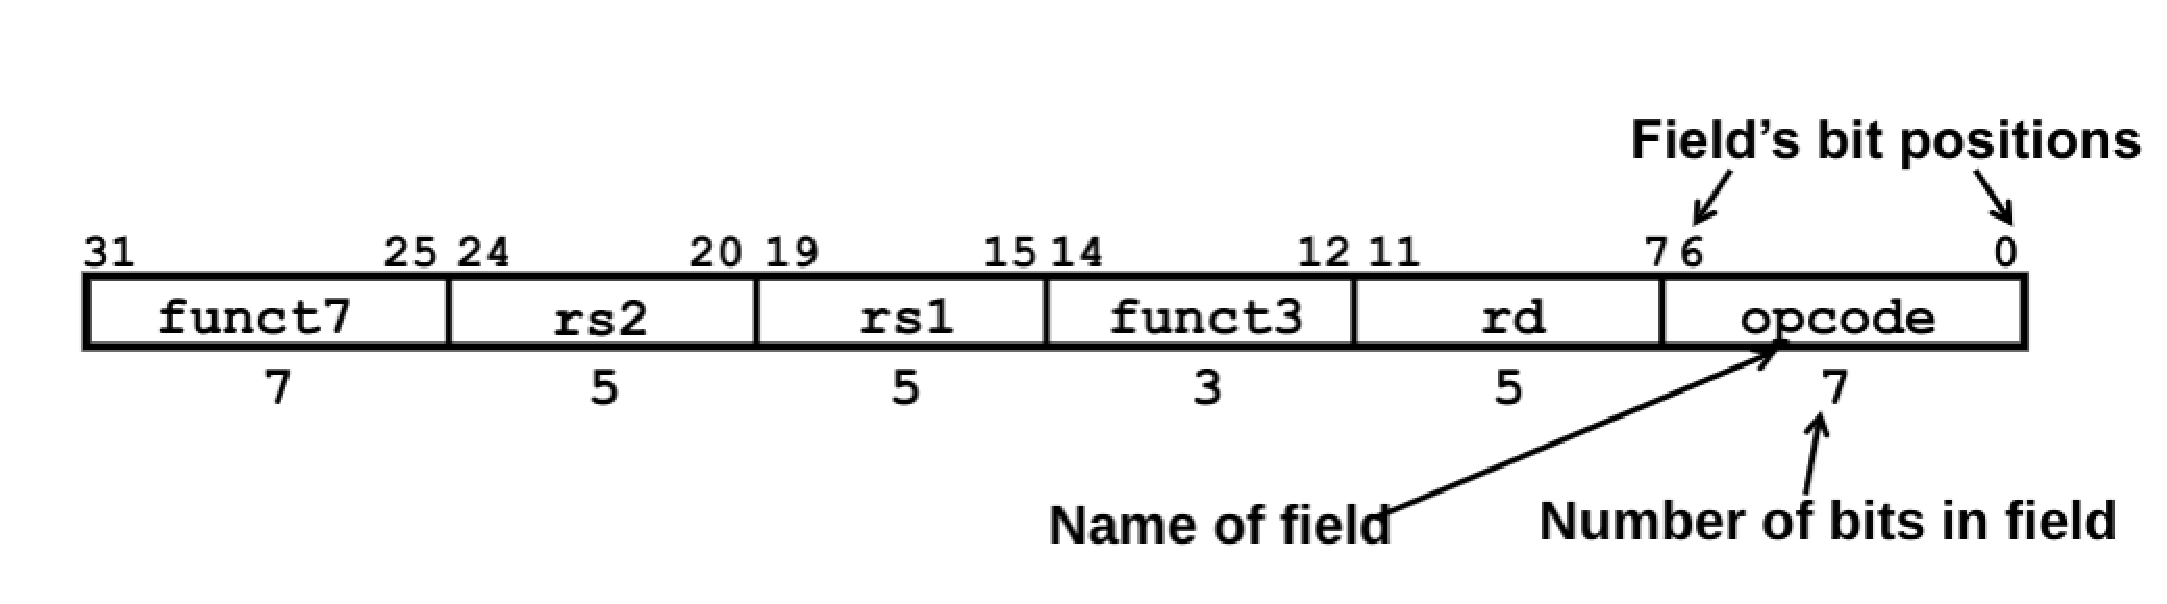
\includegraphics[width=0.8 \textwidth]{figs/RISC-V/指令表示/R-Format_Instruction_Layout.eps}
  \caption{R型指令格式的划分\\ 其中每个域中的文字表示该域的名称;域上的数字表示,该域的起始与终止位置;每个域下面的数字,表示每个域所占据的bit位数}
  \label{fig:R-Format_Instruction_Layout} %设置图形引用名称
\end{figure}
所有R指令的opcode部分都是2进制数:0110011,funct7与funct3是和opcode结合起来一起使用的,三者组合一起规定指令的操作。

rs1,rs2是源寄存器(Source Rggister),用于存放操作数的源地址的,rd是目的寄存器(Destination Rggister),指定接收结果值的寄存器编号,这三个寄存器都存放5位无符号整数(对应十进制$2^5=32$),对应0˜31的通用寄存器中的其中一个。


\subsubsection{I指令}
\textbf{I指令}是用于寄存器与立即数之间算数运算和读取的 

其实如果是我自己设计指令架构,我很有可能将操作寄存器,操作数用一个指令全部实现,但是有一个问题,就是指令中的位长,比方说R指令的源地址和目的地址才5bit,最多就能表示10进制的32位,那要是操作数字就显得有些有限;但是如果你把指令中的位长加长的话,就会造成可以表示的10进制数太多,但是寄存器就32了,造成不必要的浪费。

所以,I型指令可以在R型指令的基础上做一些稍微的改动即可,如图\ref{fig:R_I}所示。

\begin{figure}[htbp]
  \centering %居中显示
  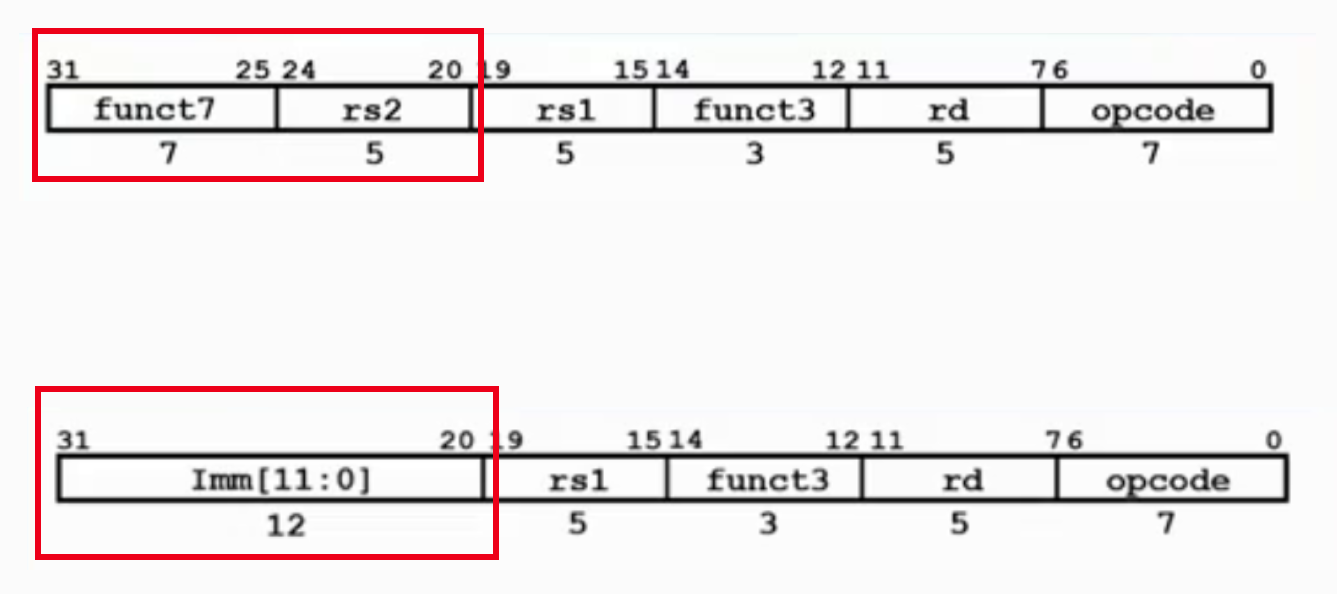
\includegraphics[width=0.8 \textwidth]{figs/RISC-V/指令表示/R_I.eps}
  \caption{I型指令就是把R型指令的前两个域合并成一个了12位的有符号数}
  \label{fig:R_I} %设置图形引用名称
\end{figure}



\subsubsection{S指令}
用于写存储器的

\subsubsection{B指令}
用于分支转移操作的,其实是S指令的一个变体,之前也叫\textbf{SB指令}

\subsubsection{U指令}
用于高20-bit位立即数操作

\subsubsection{J指令}
用于跳转操作,其实是U指令的一个变体,之前也叫\textbf{UJ指令}


\subsection{流水线}
\subsubsection{处理器性能度量方法}
首先,我认为在我们研究之前应该明确我们常说的提高性能是指什么,是表示更快的响应时间?从而更快的完成需要执行的任务?还是单位时间内能完成更多的任务?还是使用寿命更长一些?

我觉得性能的本质是——

\begin{equation}\label{eq:Computer_Analogy}
    \frac{ Time }{ Program } = \frac{ Instructions }{ Program } * \frac{ Cycles }{ Instruction } * \frac{ Time }{ Cycle }
\end{equation}

公式 (\ref{eq:Computer_Analogy})是与处理器性能有关的定理

\subsubsection{流水线的设计}
处理器执行一条指令的步骤——取指,译码,执行,访存,写回。

\subsubsection{结构冒险}
造成这个冒险的原因是硬件不支持同一周期执行多条指令

这个也比较好解决1.让其他阻塞一下等待硬件空闲下来在使用,2.要么就是多添加点硬件。



\subsubsection{数据冒险}
导致数据冒险发生简言之就是不同指令之间存在数据的关联,造成了无法提供指令执行所需的数据,进而指令不能在预期的时钟周期内执行。

解决方案就是 1.让其他阻塞一下等待数据使用完在使用,2.增加一个\textbf{旁路(bypassing)},这样的好处就是不需要等待指令完成就可以超市解决数据冒险。如图\ref{fig:Data_Hazards1} 所示,第一条add指令执行EX阶段的输出前递到sub指令的EX阶段的输入,替换sub指令在第二阶段督促的寄存器X1的值。

\begin{figure}[htbp]
  \centering %居中显示
  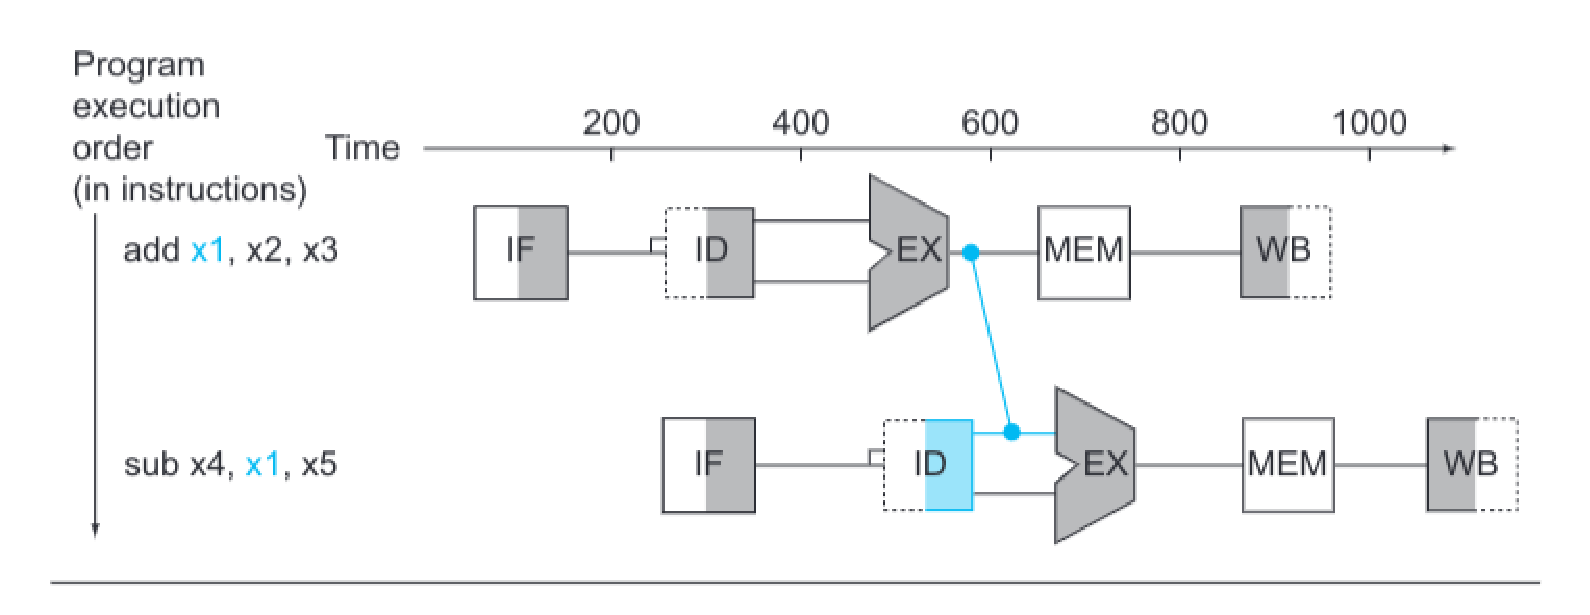
\includegraphics[width=0.8 \textwidth]{figs/RISC-V/流水线/数据冒险1.eps}
  \caption{这张图片就显示了旁路的效果}
  \label{fig:Data_Hazards1} %设置图形引用名称
\end{figure}

但是有时尽管使用了旁路,也不可避免的需要\textbf{流水线停顿(pipeline Stall)},俗称\textbf{气泡(bubble)},图\ref{fig:Data_Hazards2}就是load指令执行之后,紧跟着一条需要使用他结果的R型指令

\begin{figure}[htbp]
  \centering %居中显示
  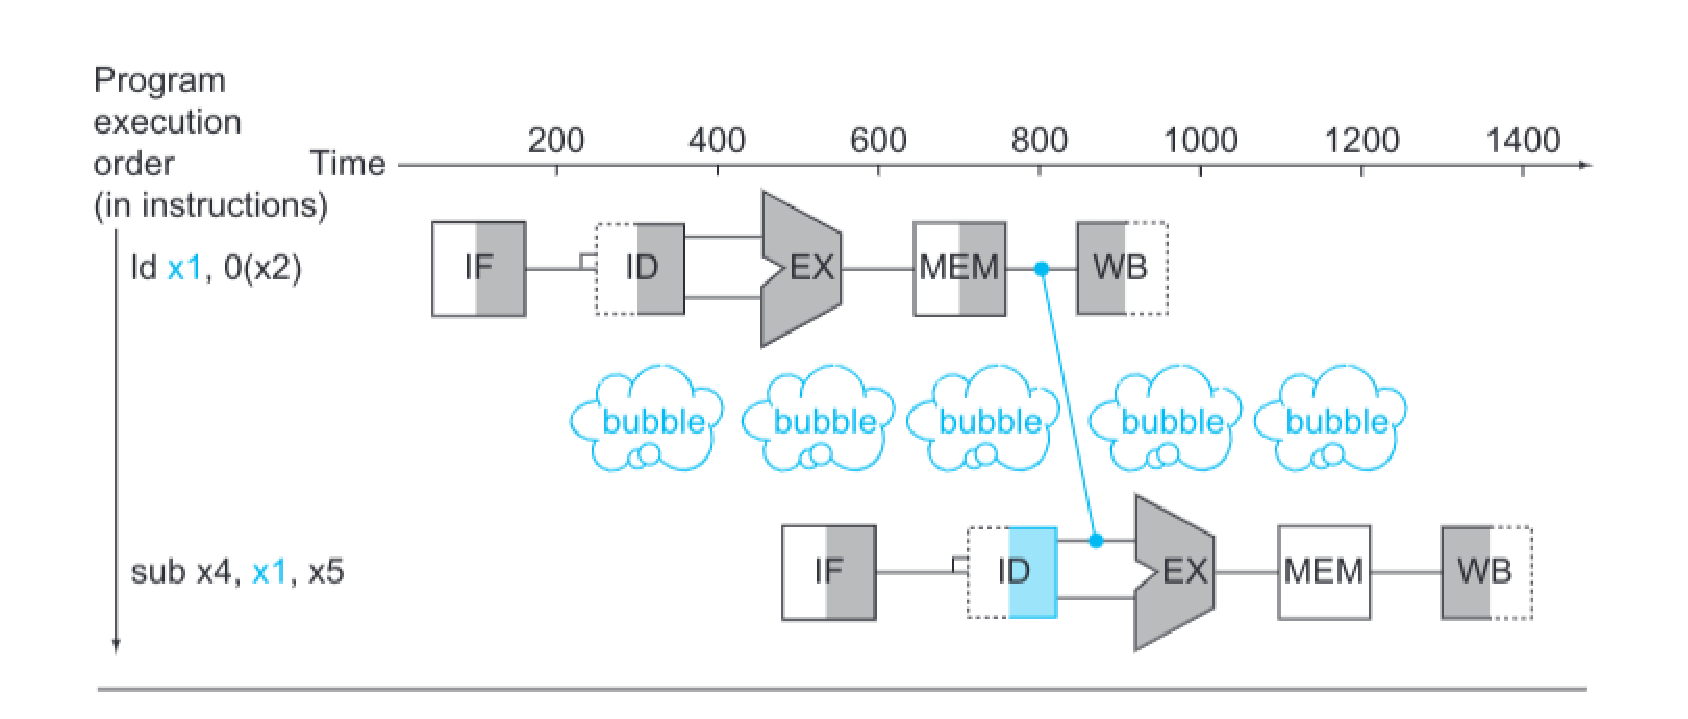
\includegraphics[width=0.8 \textwidth]{figs/RISC-V/流水线/数据冒险2.eps}
  \caption{这张就表示有时即使使用旁路,也许要阻塞等待}
  \label{fig:Data_Hazards2} %设置图形引用名称
\end{figure}


\subsubsection{控制冒险}
这种冒险发生在根据一条指令的结果判断接下来要执行的分支程序。如图\ref{fig:Control_Hazards}所示

\begin{figure}[htbp]
  \centering %居中显示
  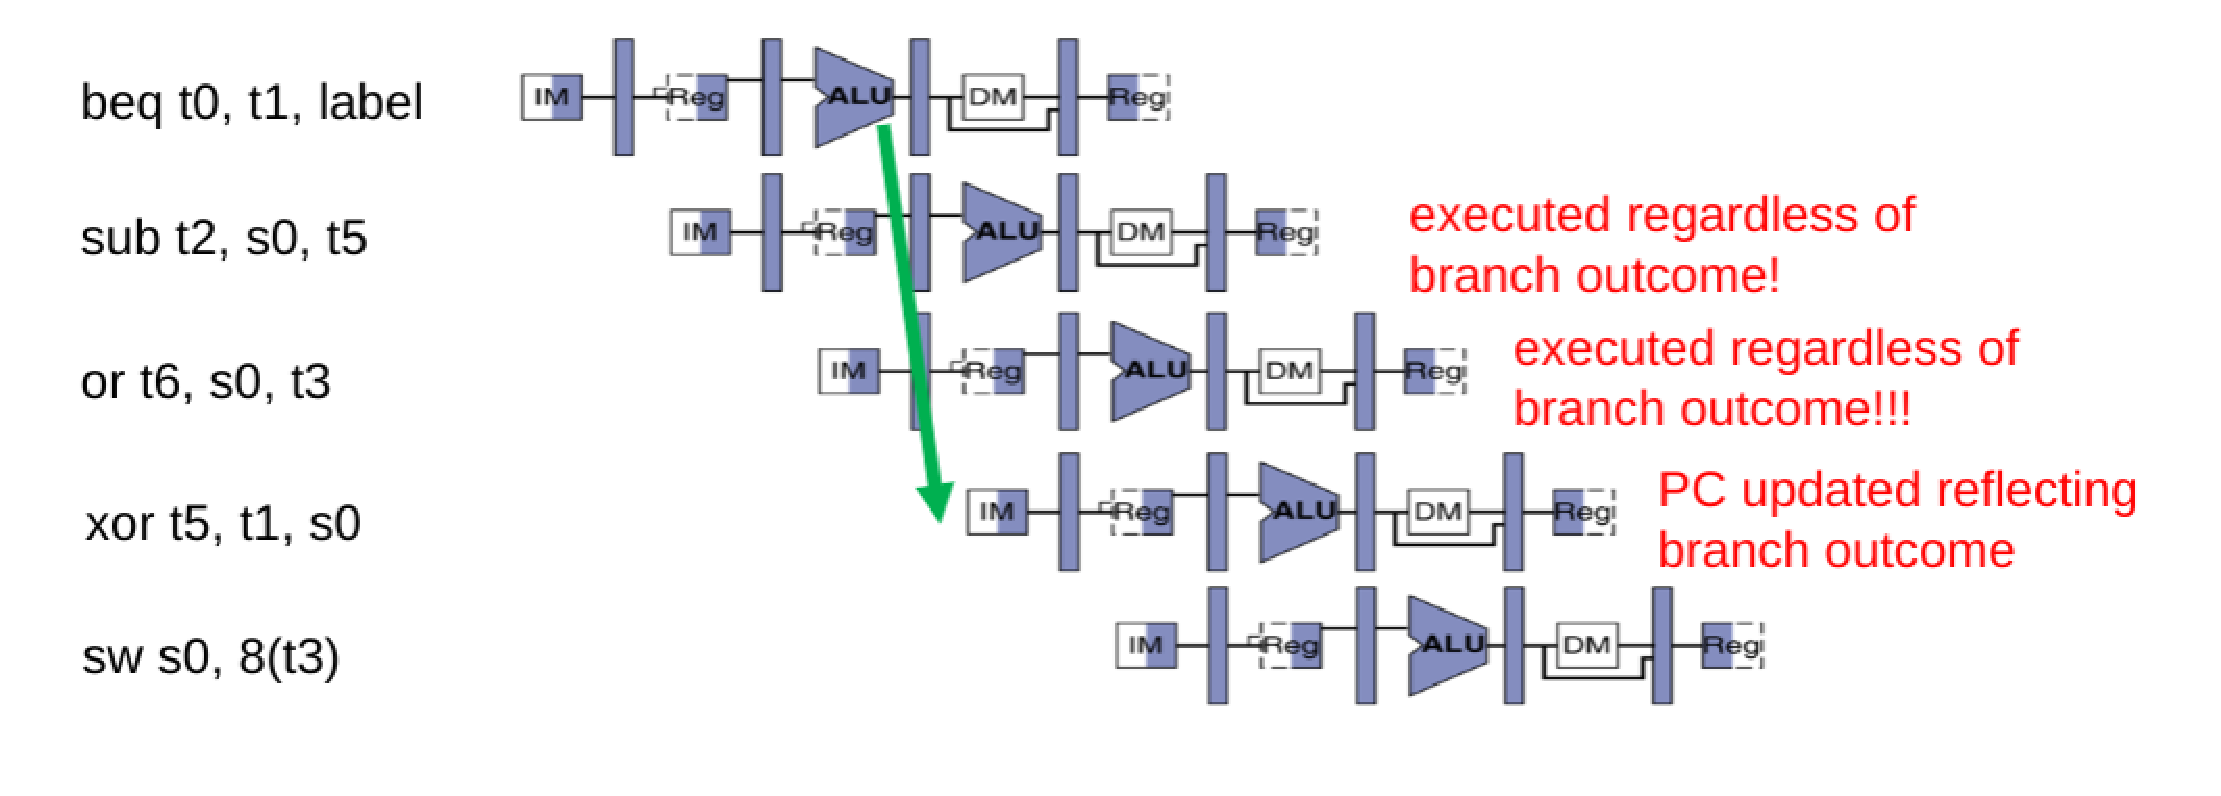
\includegraphics[width=0.8 \textwidth]{figs/RISC-V/流水线/控制冒险.eps}
  \caption{控制冒险}
  \label{fig:Control_Hazards} %设置图形引用名称
\end{figure}

解决方法1.阻塞等待,2.采用\textbf{分支预测},要是预测对了,就继续执行,如图\ref{fig:Control_Hazards_Success};如果预测错了,流水线清空刚才加载错误的指令,重新在装载正确的指令,如图\ref{fig:Control_Hazards_Fail}。

\begin{figure}[htbp]
  \centering %居中显示
  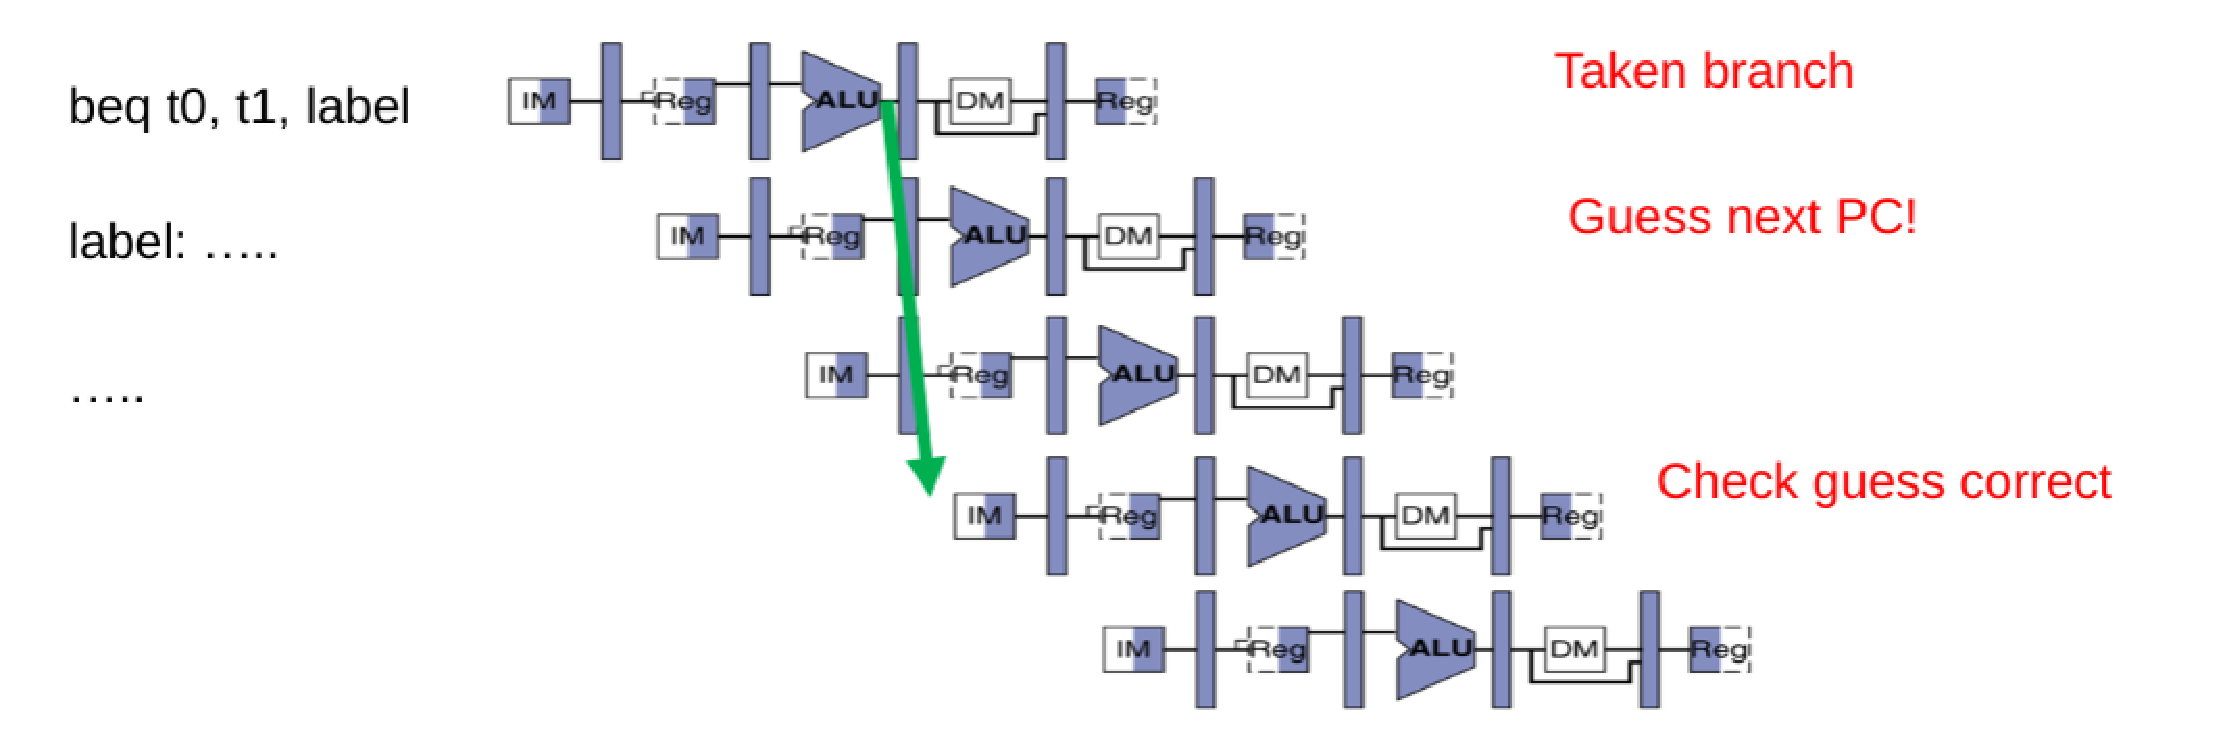
\includegraphics[width=0.8 \textwidth]{figs/RISC-V/流水线/控制冒险_预测成功.eps}
  \caption{分支预测:预测成功}
  \label{fig:Control_Hazards_Success} %设置图形引用名称
\end{figure}

\begin{figure}[htbp]
  \centering %居中显示
  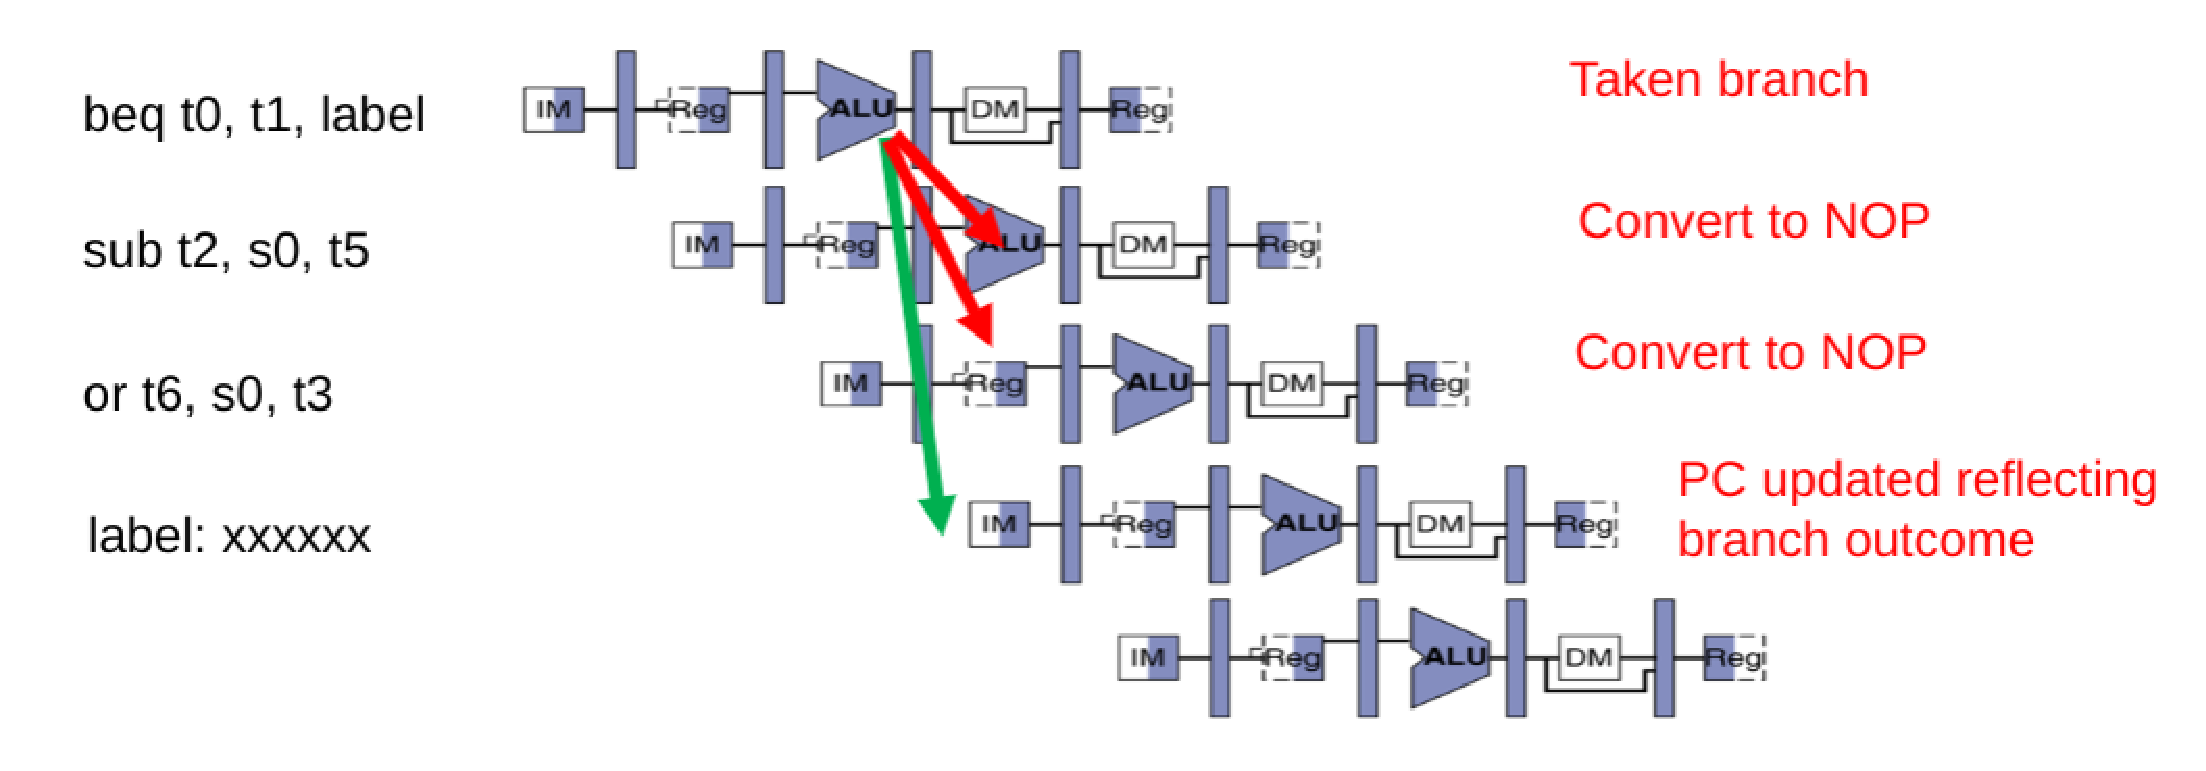
\includegraphics[width=0.8 \textwidth]{figs/RISC-V/流水线/控制冒险_预测失败.eps}
  \caption{分支预测:预测失败}
  \label{fig:Control_Hazards_Fail} %设置图形引用名称
\end{figure}







\newpage % 介绍RISC-V架构内容
% 本章节介绍Qemu的原理
\section{Qemu \& KVM 基本原理}
\subsection{虚拟化}
根据维基百科关于虚拟化的定义是:“In computing,virtualization refers to the act of creating a virtual(rather than actual)version of something,including virtual computer hardware platforms,storage devices,and computer network resources。”(在计算机领域,虚拟化指创建某事物的虚拟(而非实际)版本,包括虚拟的计算机硬件平台、存储设备,以及计算机网络资源)可见,虚拟化是一种资源管理技术,它将计算机的各种实体资源(CPU、内存、存储、网络等)予以抽象和转化出来,并提供分割、重新组合,以达到最大化利用物。

\subsubsection{软件虚拟化}
就是Qemu来实现VMM层,通过纯软件的环境来模拟执行客户机里的指令。Qemu是软件层面实现二进制翻译(二进制翻译(binary translation)是指将使用某套指令集的二进制代码转换成基于另一套指令集的。)出目标平台代码交给客户机,客户机的每一条目标平台指令都会被QEMU截取,并翻译成宿主机平台的指令,然后交给实际的物理平台执行。

\subsubsection{硬件虚拟化}
这里以x86结构为例,Intel在2005年就加入硬件虚拟化的支持——Intel VT。简单来说就是计算机硬件本身有让客户机指令独立执行的能力,不完全需要VMM截获重定向。

其实客户机在Linux上就是一个进程,客户机访问自己的物理内存,实际上就是Linux内核管理的虚拟内存,以前是使用软件实现客户机虚拟地址(GVA)到客户机物理地址(GPA)再到宿主机虚拟地址(HVA)最后到宿主机物理地址(HPA)的四步转换,这个机制也称为“影子页表”,但是执行代价很大,后来这种靠软件实现的方式被硬件逻辑取代,这就是Intel的EPT技术(或者AMD的NPT技术),靠硬件自动算出GPA到HPA的过程。

\subsection{硬件虚拟化介绍}

\subsubsection{CPU虚拟化}
Intel在处理器级别提供了对虚拟化技术的支持,被称为VMX(virtual-machine
extensions)。有两种VMX操作模式:VMX根操作(root operation)与VMX非根操作
(non-root operation)。作为虚拟机监控器中的KVM就是运行在根操作模式下,而虚拟机
客户机的整个软件栈(包括操作系统和应用程序)则运行在非根操作模式下。进入VMX
非根操作模式被称为“VM Entry”;从非根操作模式退出,被称为“VM Exit”。

VMX的根操作模式与非VMX模式下最初的处理器执行模式基本一样,只是它现在支
持了新的VMX相关的指令集以及一些对相关控制寄存器的操作。VMX的非根操作模式是
一个相对受限的执行环境,为了适应虚拟化而专门做了一定的修改;在客户机中执行的一
些特殊的敏感指令或者一些异常会触发“VM Exit”退到虚拟机监控器中,从而运行在VMX
根模式。正是这样的限制,让虚拟机监控器保持了对处理器资源的控制。

一个虚拟机监控器软件的最基础的运行生命周期及其与客户机的交互如图 \ref{fig:VMM_Guest} 所示。
\begin{figure}[htbp]
    \centering
    \def\svgwidth{\columnwidth}
    \import{./figs/RISC-V/KVM/VMM_Guest/}{VMM_Guest.pdf_tex}
    \caption{VMM与Guest之间的交互}
    \label{fig:VMM_Guest}
\end{figure}
软件通过执行VMXON指令进入VMX操作模式下;在VMX模式下通过VMLAUNCH和VMRESUME指令进入客户机执行模式,即VMX非根模式;当在非根模式下触发VM Exit时,处理器执行控制权再次回到宿主机的虚拟机监控器上;最后虚拟机监控可以执行VMXOFF指令退出VMX执行模式。

逻辑处理器在根模式和非根模式之间的切换通过一个叫作VMCS(virtual-machinecontrol data structure)的数据结构来控制;而VMCS的访问是通过VMCS指针来操作的。VMCS指针是一个指向VMCS结构的64位的地址,使用VMPTRST和VMPTRLD指令对VMCS指针进行读写,使用MREAD、VMWRITE和VMCLEAR等指令对VMCS实现配置。

对于一个逻辑处理器,它可以维护多个VMCS数据结构,但是在任何时刻只有一个VMCS在当前真正生效。多个VMCS之间也是可以相互切换的,VMPTRLD指令就让某个VMCS在当前生效,而其他VMCS就自然成为不是当前生效的。一个虚拟机监控器会为一个虚拟客户机上的每一个逻辑处理器维护一个VMCS数据结构。

\subsubsection{内存虚拟化}
内存虚拟化的目的是给虚拟客户机操作系统提供一个从0地址开始的连续物理内存空间,同时在多个客户机之间实现隔离和调度。

在虚拟环境下内存地址如图 \ref{fig:Virtual2Physical_Address} 所示。
\begin{figure}[htbp]
    \centering
    \def\svgscale{0.5}
    \import{./figs/RISC-V/KVM/Virtual2Physical_Address/}{Virtual2Physical_Address.pdf_tex}
    \caption{虚拟化环境下的内存地址}
    \label{fig:Virtual2Physical_Address}
\end{figure}

内存虚拟化就是要将客户机虚拟地址(GVA)转化为最终能够访问的宿主机上的物理地址(HPA)。对于客户机操作系统而言,它不感知内存虚拟化的存在,在程序访问客户机中虚拟地址时,通过CR3寄存器可以将其转化为物理地址,但是在虚拟化环境中这个物理地址只是客户机的物理地址,还不是真实内存硬件上的物理地址。所以,虚拟机监控器就需要维护从客户机虚拟地址到宿主机物理地址之间的一个映射关系,在没有硬件提供的内存虚拟化之前,这个维护映射关系的页表叫作影子页表(Shadow Page Table)。内存的访问和更新通常是非常频繁的,要维护影子页表中对应关系会非常复杂,开销也较大。同时需要为每一个客户机都维护一份影子页表,当客户机数量较多时,其影子页表占用的内存较大也会是一个问题。

Intel CPU在硬件设计上就引入了EPT(Extended Page Tables,扩展页表),从而将客户机虚拟地址到宿主机物理地址的转换通过硬件来实现。当然,这个转换是通过两个步骤来实现的,如图2-3所示。首先,通过客户机CR3寄存器将客户机虚拟地址转化为客户机物理地址,然后通过查询EPT来实现客户机物理地址到宿主机物理地址的转化。EPT的控制权在虚拟机监控器中,只有当CPU工作在非根模式时才参与内存地址的转换。使用EPT后,客户机在读写CR3和执行INVLPG指令时不会导致VM Exit,而且客户页表结构自身导致的页故障也不会导致VM Exit。所以通过引入硬件上EPT的支持,简化了内存虚拟化的实现复杂度,同时也提高了内存地址转换的效率。


\subsubsection{I/O虚拟化}
在虚拟化的架构下,虚拟机监控器必须支持来自客户机的I/O请求。通常情况下有以下4种I/O虚拟化方式。
1)设备模拟:在虚拟机监控器中模拟一个传统的I/O设备的特性,比如在QEMU中模拟一个Intel的千兆网卡或者一个IDE硬盘驱动器,在客户机中就暴露为对应的硬件设备。客户机中的I/O请求都由虚拟机监控器捕获并模拟执行后返回给客户机。

2)前后端驱动接口:在虚拟机监控器与客户机之间定义一种全新的适合于虚拟化环境的交互接口,比如常见的virtio协议就是在客户机中暴露为virtio-net、virtio-blk等网络和磁盘设备,在QEMU中实现相应的virtio后端驱动。

3)设备直接分配:将一个物理设备,如一个网卡或硬盘驱动器直接分配给客户机使用,这种情况下I/O请求的链路中很少需要或基本不需要虚拟机监控器的参与,所以性能很好。

4)设备共享分配:其实是设备直接分配方式的一个扩展。在这种模式下,一个(具有特定特性的)物理设备可以支持多个虚拟机功能接口,可以将虚拟功能接口独立地分配给不同的客户机使用。如SR-IOV就是这种方式的一个标准协议。

表\ref{fig:I/O_virtual}展示了这4种I/O虚拟化方式的优缺点,前两种都是纯软件的实现,后两种都需要特定硬件特性的支持。

% 插入表格
\begin{table}[htbp]
     \centering
\begin{tabular}{|c|l|l|}
\hline
\multicolumn{1}{|l|}{} & \textbf{优点}                                                 & \textbf{缺点}                                                                              \\ \hline
设备模拟                   & 兼容性好,不需要额外驱动                                                & \begin{tabular}[c]{@{}l@{}}1.性能较差\\ 2.模拟设备的功能特性支持不够多\end{tabular}                        \\ \hline
前后端接口                  & 性能有所提升                                                      & \begin{tabular}[c]{@{}l@{}}1.兼容性差一些:依赖客户机总安装特定驱动\\ 2.I/O压力大时,后端驱动的CPU资源占用较高\end{tabular} \\ \hline
设备直接分配                 & 性能非常好                                                       & \begin{tabular}[c]{@{}l@{}}1.需要硬件设备的特性支持\\ 2.单个设备只能分配一个客户机\\ 3.很难支持动态迁移\end{tabular}     \\ \hline
设备共享分配                 & \begin{tabular}[c]{@{}l@{}}1.性能非常好\\ 2.单个设备可共享\end{tabular} & \begin{tabular}[c]{@{}l@{}}1.所需设备硬件的特性支持\\ 2.很难支持动态迁移\end{tabular}                       \\ \hline
\end{tabular}
\caption{常见I/O虚拟化方式的优缺点}
\label{fig:I/O_virtual}
\end{table}


\subsection{KVM \& Qemu模拟器介绍}
首先Qemu(Quick Emulator)本身并不完全是KVM的一部分,它是一套由软件模拟实现的。

而KVM(Kernel Virtual Machine)是有两部分组成,一部分是Linux内核的KVM模块,另一块是经过简化后的Qemu。它能够让Linux主机成为一个Hypervisor(虚拟机监控器)。在支持VMX(Virtual    Machine Extension)功能的x86处理器中,Linux在原有的用户模式和内核模式中新增加了客户模式,并且客户模式也拥有自己的内核模式和用户模式,虚拟机就是运行在客户模式中。三层结构如   图\ref{fig:kvm}所示。

\begin{figure}[htbp]
    \centering
    \def\svgscale{0.5}
    \import{./figs/RISC-V/KVM/KVM_3model/}{kvm_3model.pdf_tex}
    \caption{KVM三种模式的层次关系}
    \label{fig:kvm}
\end{figure}    
%『h』当前位置。将图形放置在正文文本中给出该图形环境的地方。如果本页所剩的页面不够,这一参数将不起作用。
%『t』顶部。将图形放置在页面的顶部。
%『b』底部。将图形放置在页面的底部。
%『p』浮动页。将图形放置在一只允许有浮动对象的页面上。

KVM就是在硬件辅助虚拟化技术之上构建起来的虚拟机监控器。

当然,并非要所有这些硬件虚拟化都支持才能运行KVM虚拟化,KVM对硬件最低的依赖是CPU的硬件虚拟化支持。

\subsubsection{KVM内核模块}
KVM模块是KVM虚拟化的核心模块,它在内核中由两部分组成:一个是处理器架构无关的部分,用lsmod命令中可以看到,如图 \ref{fig:lsmod_kvm} 所示,叫作kvm模块;另一个是处理器架构相关的部分,在Intel平台上就是$kvm\_intel$这个内核模块。KVM的主要功能是初始化CPU硬件,打开虚拟化模式,然后将虚拟客户机运行在虚拟机模式下,并对虚拟客户机的运行提供一定的支持。

\begin{figure}[htbp]
  \centering %居中显示
  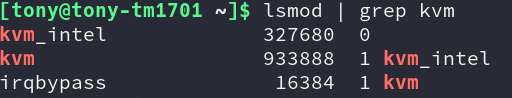
\includegraphics[width=0.9 \textwidth]{figs/RISC-V/KVM/lsmod_kvm.png}
  \caption{lsmod}
  \label{fig:lsmod_kvm} %设置图形引用名称
\end{figure}

以KVM在Intel公司的CPU上运行为例,在被内核加载的时候,KVM模块会先初始化内部的数据结构;做好准备之后,KVM模块检测系统当前的CPU,然后打开CPU控制寄存器CR4中的虚拟化模式开关,并通过执行VMXON指令将宿主操作系统(包括KVM模块本身)置于CPU执行模式的虚拟化模式中的根模式;最后,KVM模块创建特殊设备文件/dev/kvm并等待来自用户空间的命令。接下来,虚拟机的创建和运行将是一个用户空间的应用程序(QEMU)和KVM模块相互配合的过程。

/dev/kvm这个设备可以被当作一个标准的字符设备,KVM模块与用户空间QEMU的通信接口主要是一系列针对这个特殊设备文件的loctl调用。当然,每个虚拟客户机针对/dev/kvm文件的最重要的loctl调用就是“创建虚拟机”。在这里,“创建虚拟机”可以理解成KVM为了某个特定的虚拟客户机(用户空间程序创建并初始化)创建对应的内核数据结构。同时,KVM还会返回一个文件句柄来代表所创建的虚拟机。针对该文件句柄的loctl调用可以对虚拟机做相应的管理,比如创建用户空间虚拟地址和客户机物理地址及真实内存物理地址的映射关系,再比如创建多个可供运行的虚拟处理器(vCPU)。同样,KVM模块会为每一个创建出来的虚拟处理器生成对应的文件句柄,对虚拟处理器相应的文件句柄进行相应的loctl调用,就可以对虚拟处理器进行管理。

针对虚拟处理器的最重要的loctl调用就是“执行虚拟处理器”。通过它,用户空间准备好的虚拟机在KVM模块的支持下,被置于虚拟化模式中的非根模式下,开始执行二进制指令。在非根模式下,所有敏感的二进制指令都会被处理器捕捉到,处理器在保存现场之后自动切换到根模式,由KVM决定如何进一步处理(要么由KVM模块直接处理,要么返回用户空间交由用户空间程序处理)。

除了处理器的虚拟化,内存虚拟化也是由KVM模块实现的,包括前面提到的使用硬件提供的EPT特性,通过两级转换实现客户机虚拟地址到宿主机物理地址之间的转换。

处理器对设备的访问主要是通过I/O指令和MMIO,其中I/O指令会被处理器直接截获,MMIO会通过配置内存虚拟化来捕捉。但是,外设的模拟一般不由KVM模块负责。一般来说,只有对性能要求比较高的虚拟设备才会由KVM内核模块来直接负责,比如虚拟中断控制器和虚拟时钟,这样可以大量减少处理器模式切换的开销。而大部分的输入输出设备交给下一节将要介绍的用户态程序QEMU来负责。

\subsubsection{QEMU用户态设备模拟}
QEMU原本就是一个著名的开源虚拟机软件项目,而不是KVM虚拟化软件的一部分。与KVM不同,QEMU最初实现的虚拟机是一个纯软件的实现,通过二进制翻译来实现虚拟化客户机中的CPU指令模拟,所以性能比较低。但是,其优点是跨平台,QEMU支持在Linux、Windows、FreeBSD、Solaris、MacOS等多种操作系统上运行,能支持在QEMU本身编译运行的平台上就实现虚拟机的功能,甚至可以支持客户机与宿主机并不是同一个架构(比如在x86平台上运行ARM客户机)。作为一个存在已久的虚拟机监控器软件,QEMU的代码中有完整的虚拟机实现,包括处理器虚拟化、内存虚拟化,以及KVM也会用到的虚拟设备模拟(比如网卡、显卡、存储控制器和硬盘等)。

除了二进制翻译的方式,QEMU也能与基于硬件虚拟化的Xen、KVM结合,为它们提供客户机的设备模拟。通过与KVM的密切结合,让虚拟化的性能提升得非常高,在真实的企业级虚拟化场景中发挥重要作用,所以我们通常提及KVM虚拟化时就会说“QEMU/KVM”这样的软件栈。

最早期的KVM开发者们为了简化软件架构和代码重用,根据KVM特性在QEMU的基础上进行了修改(当然这部分修改已经合并回QEMU的主干代码,故现在的QEMU已原生支持KVM虚拟化特性)。从图2-8可以看出,每一个虚拟客户机在宿主机中就体现为一个QEMU进程,而客户机的每一个虚拟CPU就是一个QEMU线程。虚拟机运行期间,QEMU会通过KVM模块提供的系统调用进入内核,由KVM模块负责将虚拟机置于处理器的特殊模式下运行。遇到虚拟机进行I/O操作时,KVM模块会从上次的系统调用出口处返回QEMU,由QEMU来负责解析和模拟这些设备。

从QEMU角度来看,也可以说QEMU使用了KVM模块的虚拟化功能,为自己的虚拟机提供硬件虚拟化的加速,从而极大地提高了虚拟机的性能。除此之外,虚拟机的配置和创建,虚拟机运行依赖的虚拟设备,虚拟机运行时的用户操作环境和交互,以及一些针对虚拟机的特殊技术(如:动态迁移),都是由QEMU自己实现的。

QEMU除了提供完全模拟的设备(如:e1000网卡、IDE磁盘等)以外,还支持virtio协议的设备模拟。virtio是一个沟通客户机前端设备与宿主机上设备后端模拟的比较高性能的协议,在前端客户机中需要安装相应的virtio-blk、virtio-scsi、virtio-net等驱动,而QEMU就实现了virtio的虚拟化后端。QEMU还提供了叫作virtio-blk-data-plane的一种高性能的块设备I/O方式,它最初在QEMU 1.4版本中被引入。virtio-blk-data-plane与传统virtio-blk相比,它为每个块设备单独分配一个线程用于I/O处理,data-plane线程不需要与原QEMU执行线程同步和竞争锁,而且它使用ioeventfd/irqfd机制,同时利用宿主机Linux上的AIO(异步I/O)来处理客户机的I/O请求,使得块设备I/O效率进一步提高。

总之,QEMU既是一个功能完整的虚拟机监控器,也在QEMU/KVM的软件栈中承担设备模拟的工作。


\subsection{KVM上层管理工具}

\subsubsection{libvirt}
libvirt是使用最广泛的对KVM虚拟化进行管理的工具和应用程序接口,已经是事实上的虚拟化接口标准,本节后部分介绍的其他工具都是基于libvirt的API来实现的。作为通用的虚拟化API,libvirt不但能管理KVM,还能管理VMware、Hyper-V、Xen、VirtualBox等其他虚拟化方案。

\subsubsection{virsh}
virsh是一个常用的管理KVM虚拟化的命令行工具,对于系统管理员在单个宿主机上进行运维操作,virsh命令行可能是最佳选择。virsh是用C语言编写的一个使用libvirt API的虚拟化管理工具,其源代码也是在libvirt这个开源项目中的。

\subsubsection{virt-manager}
virt-manager是专门针对虚拟机的图形化管理软件,底层与虚拟化交互的部分仍然是调用libvirt API来操作的。virt-manager除了提供虚拟机生命周期(包括:创建、启动、停止、打快照、动态迁移等)管理的基本功能,还提供性能和资源使用率的监控,同时内置了VNC和SPICE客户端,方便图形化连接到虚拟客户机中。virt-manager在RHEL、CentOS、Fedora等操作系统上是非常流行的虚拟化管理软件,在管理的机器数量规模较小时,virt-manager是很好的选择。因其图形化操作的易用性,成为新手入门学习虚拟化操的首选管理软件。












\newpage %介绍Qemu模拟器的原理
% 本章节是介绍实验流程
\section{实验流程}
本实验是参考Github上的项目 \cite{BusyBear} 来实现的。

\subsection{实验平台}
本实验环境是在 x86 平台,基于linux环境进行的,具体信息如图\ref{fig:gentoo} 

\begin{figure}[htbp]
  \centering %居中显示
  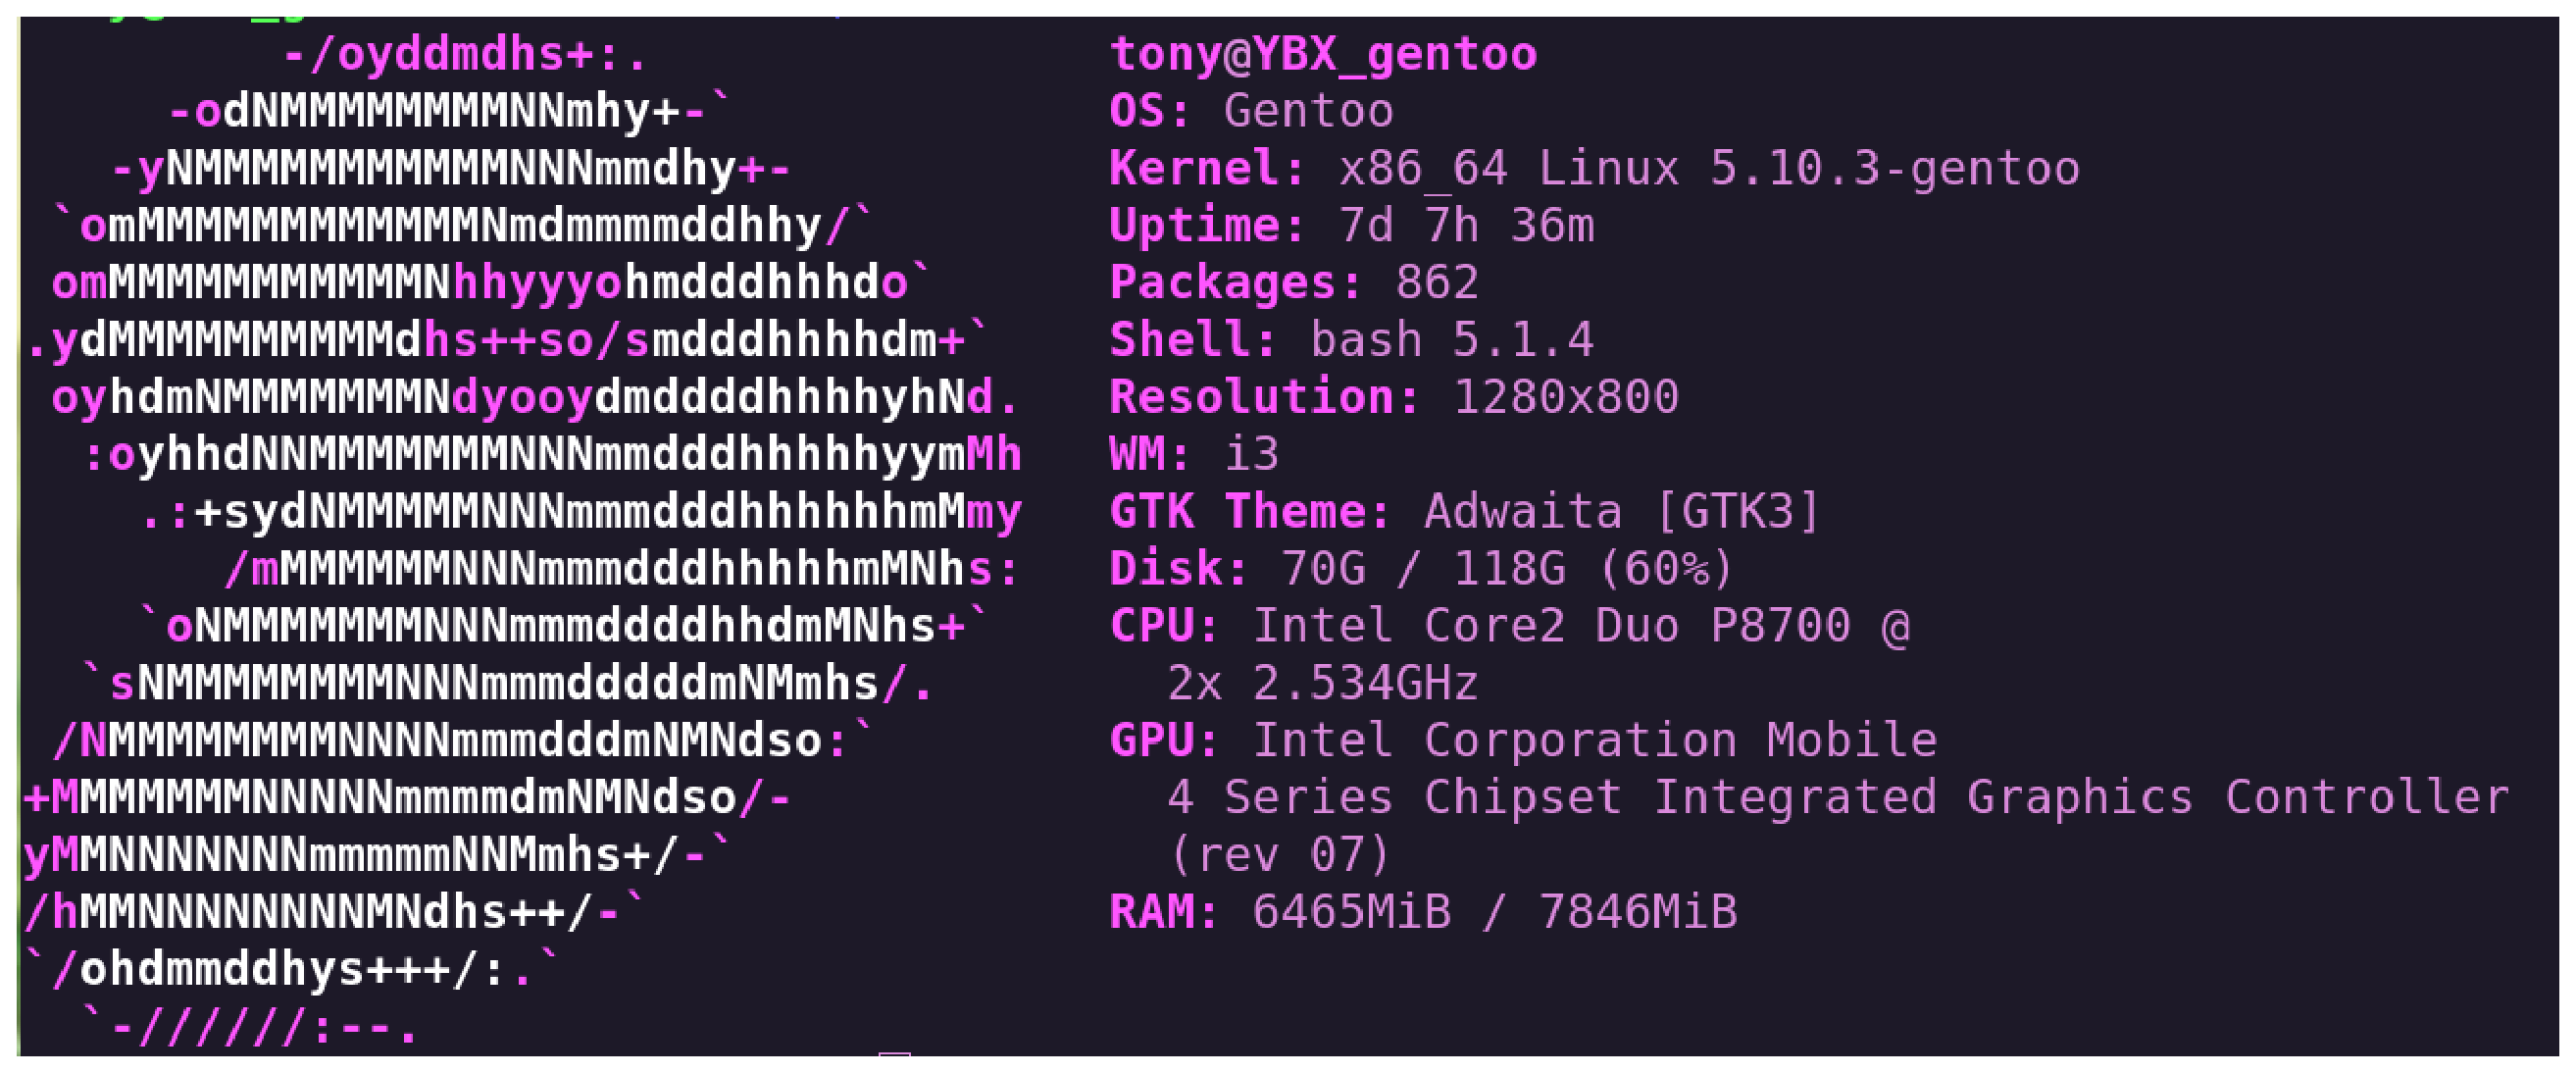
\includegraphics[width=0.6 \textwidth]{figs/gentoo_Logo.eps}
  \caption{实验操作系统}
  \label{fig:gentoo} %设置图形引用名称
\end{figure}

\subsection{Qemu搭建}
在 Gentoo 官方的 Wiki 手册中可以参考 \cite{GentooQemu}
\subsubsection{检测处理器是否支持虚拟化}
\begin{lstlisting}
\$ grep --color -E "vmx|svm" /proc/cpuinfo 
\end{lstlisting}
如果能显示出 图\ref{fig:vmx_svm} 说明处理器是支持虚拟化的

\begin{figure}[htbp]
  \centering %居中显示
  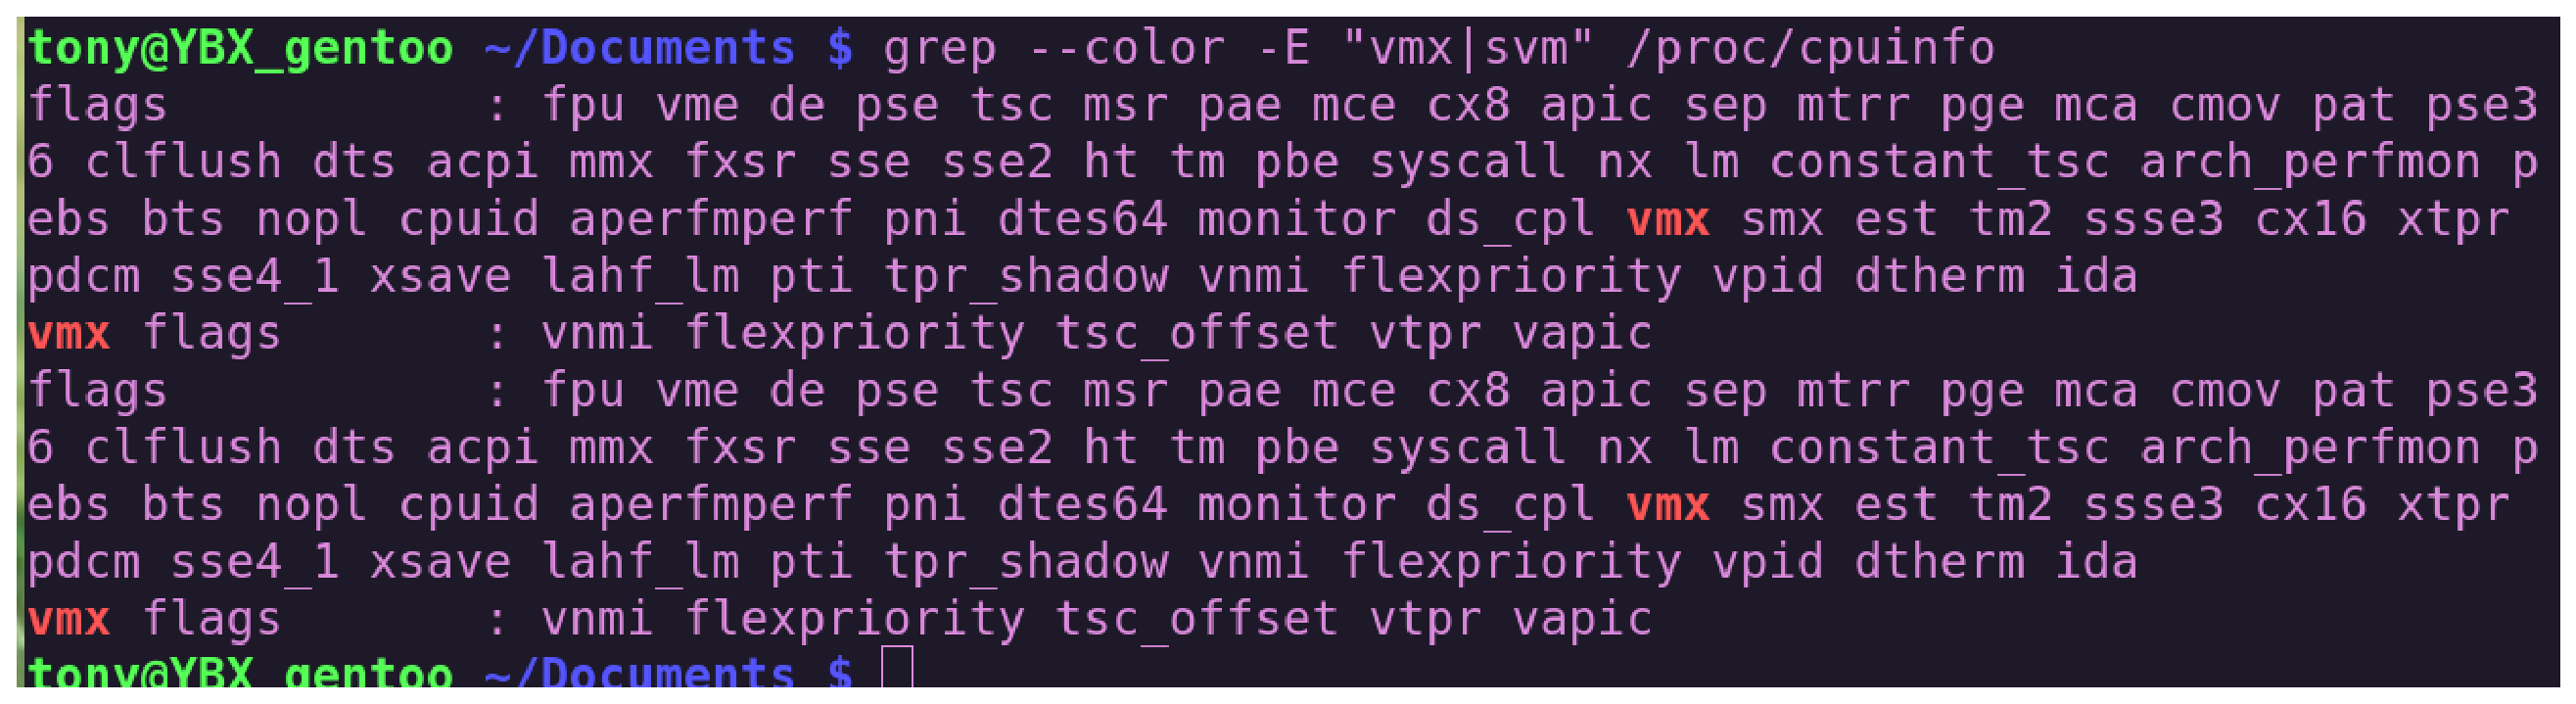
\includegraphics[width=0.6 \textwidth]{figs/vmx_svm.eps}
  \caption{是否支持虚拟化}
  \label{fig:vmx_svm} %设置图形引用名称
\end{figure}

\subsubsection{编译内核}
首先需要更改内核配置

\begin{lstlisting}
cd /usr/src/linux
make menuconfig 
\end{lstlisting}

然后根据以下步骤进行配置内核,使其支持KVM,其中 图\ref{fig:KVM_Intel} 是根据自己处理器来选择的,我的是Intel的处理器,如果使用AMD处理器的话,需要勾选另一个。

\begin{figure}[htbp]
  \centering %居中显示
  \includegraphics[width=0.9 \textwidth]{figs/Kernel/Step1.eps}
  \caption{Virtualization}
  \label{fig:Virtualization} %设置图形引用名称
\end{figure}

\begin{figure}[htbp]
  \centering %居中显示
  \includegraphics[width=0.9 \textwidth]{figs/Kernel/Step2.eps}
  \caption{Kernel-based Virtual Machine (KVM) support}
  \label{fig:Kernel-based} %设置图形引用名称
\end{figure}

\begin{figure}[htbp]
  \centering %居中显示
  \includegraphics[width=0.9 \textwidth]{figs/Kernel/Step3.eps}
  \caption{KVM for Intel processors support}
  \label{fig:KVM_Intel} %设置图形引用名称
\end{figure}

\subsubsection{修改USE Flags并安装}
\begin{lstlisting}
# vim /etc/portage/make.conf
QEMU_SOFTMMU_TARGETS="riscv32 risc64"
QEMU_USER_TARGETS="x86_64"

# vim /etc/portage/package.use
app-emulation/qemu qemu_softmmu_targets_arm qemu_softmmu_targets_x86_64 qemu_softmmu_targets_sparc
app-emulation/qemu qemu_user_targets_x86_64

% 进行安装
# emerge --ask app-emulation/qemu -y
\end{lstlisting}

\subsection{简便方法}
这个步骤是比较偷懒的方式,你可以直接下载网上已经提供编译好而且运行没问题的二进制包,直接运行,但是我下载了,就没运行成功,所以就没有截图演示。
\begin{lstlisting}
cd release
wget https://github.com/michaeljclark/busybear-linux/releases/download/v1.0/bbl.bz2
wget https://github.com/michaeljclark/busybear-linux/releases/download/v1.0/busybear.bin.bz2
bzip2 -d *.bz2
\end{lstlisting}

\subsection{安装GNU工具链}

\begin{lstlisting}
mkdir YBX-bishe
cd YBX-bishe/
# 拉取 gnu-toolchain
git clone --recursive https://github.com/riscv/riscv-gnu-toolchain

# 编译生成 RISC-V newlib & Linux toolchains
cd riscv-gnu-toolchain
./configure --prefix=/opt/riscv --enable-multilib
make newlib -j5
make linux -j5
export PATH=$PATH:/opt/riscv/bin
export RISCV=/opt/risc
$
\end{lstlisting}

\subsection{创建根文件系统}
\begin{lstlisting}
cd ..
git clone https://github.com/michaeljclark/busybear-linux.git
cd busybear-linux
make -j5
\end{lstlisting}

但是这没完,因为busybear会自动帮你下载好 busybox 但是需要自己进行解压和编译

\begin{lstlisting}
CROSS_COMPILE=riscv{{bits}}-unknown-linux-gnu- make menuconfig
CROSS_COMPILE=riscv{{bits}}-unknown-linux-gnu- make
\end{lstlisting}

下面咱们就要制做最小文件系统
\begin{lstlisting}
qemu-img create rootfs.img  1g
mkfs.ext4 rootfs.img
mkdir rootfs
sudo mount -o loop rootfs.img  rootfs
cd rootfs
sudo cp -r ../busyboxsource/_install/* .
sudo mkdir proc sys dev etc etc/init.d
cd etc/init.d/
sudo touch rcS
sudo vi rcS
#!/bin/sh
mount -t proc none /proc
mount -t sysfs none /sys
/sbin/mdev -s

sudo mod +x rcS
sudo umount rootfs
\end{lstlisting}

\subsection{构建Linux内核}
\begin{lstlisting}
git clone https://github.com/torvalds/linux
cd linux
git checkout v5.4
make ARCH=riscv CROSS_COMPILE=riscv64-unknown-linux-gnu- defconfig
make ARCH=riscv CROSS_COMPILE=riscv64-unknown-linux-gnu-
\end{lstlisting}

\subsection{制作BootLoader——BBL(Berkeley Boot Loader)}
\begin{lstlisting}
cd..
git clone https://github.com/riscv/riscv-pk.git
cd riscv-pk
mkdir build
cd build
../configure --enable-logo --host=riscv64-unknown-elf --with-payload=../../riscv-linux/vmlinux
make -j8
\end{lstlisting}

\subsection{运行}
\begin{lstlisting}
cd ..
mkdir Running
cd Running
\end{lstlisting}
创建KVM启动脚本
\begin{lstlisting}
vim open_kvm
#!/bin/sh
sudo /etc/init.d/libvirtd start
sudo virsh net-start default  #开启网络服务
\end{lstlisting}

创建KVM关闭脚本
\begin{lstlisting}
sudo virsh net-destory default
sudo /etc/init.d/libvirtd stop
\end{lstlisting}


创建网络启动脚本
\begin{lstlisting}
#!/bin/sh
brctl addif virbr0 $1
ifconfig $1 up
\end{lstlisting}

创建网络关闭脚本
\begin{lstlisting}
#!/bin/sh
ifconfig $1 down
brctl delif virbr0 $1
\end{lstlisting}

创建程序运行脚本
\begin{lstlisting}
#!/bin/sh
# QEMU 5.2以后.模拟器内部集成了OpenSBI
sudo qemu-system-riscv64 \
  -nographic -machine virt \
  -m 1024M \
  -kernel bbl \
  -kernel /home/tony/Documents/Risc-v/busybear-linux/build/linux-5.0/arch/riscv/boot/Image \
  -drive file=busybear.bin,format=raw,id=hd0 \
  -device virtio-blk-device,drive=hd0 \
  -device virtio-net-device,netdev=net0 \
  -netdev type=tap,script=./ifup.sh,downscript=./ifdown.sh,id=net0 \
  -append "root=/dev/vda ro console=ttyS0" 
\end{lstlisting}






\subsection{最终效果}
最终结果演示可以看 \cite{结果演示} 



\newpage % 相关工作
% 性能评估
% 本章节介绍与前人的比较
\section{与前人比较}
\newpage  %与前人比较



%% 参考文献
\bibliographystyle{plain}
\bibliography{Ref}
%\bibliographystyle{plain}指定参考文献的呈现方式,常见的预设样式的可选项有8种,分别是:
%% 1. plain,按字母的顺序排列,比较次序为作者、年度和标题;
%% 2. unsrt,样式同plain,只是按照引用的先后排序;
%% 3. alpha,用作者名首字母+年份后两位作标号,以字母顺序排序;
%% 4. abbrv,类似plain,将月份全拼改为缩写,更显紧凑;
%% 5. ieeetr,国际电气电子工程师协会期刊样式;
%% 6. acm,美国计算机学会期刊样式;
%% 7. siam,美国工业和应用数学学会期刊样式;
%% 8. apalike,美国心理学学会期刊样式;
\end{document}
